\documentclass[accentcolor=tud6b,colorbacktitle,inverttitle,landscape,german,presentation,t]{tudbeamer}
\usepackage{ngerman}

\usepackage[utf8]{inputenc}

\begin{document}
	
	\title[Service Discovery in Distributed Mesh-Networks]{Service Discovery in Distributed Mesh-Networks}
	\subtitle{BSc Praktikum SoSe 2016}
	
	\author{Ana Barroso, Ian Bierlich, Marco Holz, Andreas Rammhold, Martin Weinelt}
	\institute{Chaos Darmstadt e.V.}

	%\logo{\url{darmstadt.freifunk.net}}

	\date{13. April 2016}
	
	\begin{titleframe}
		\begin{center}
			\vspace{1cm}
			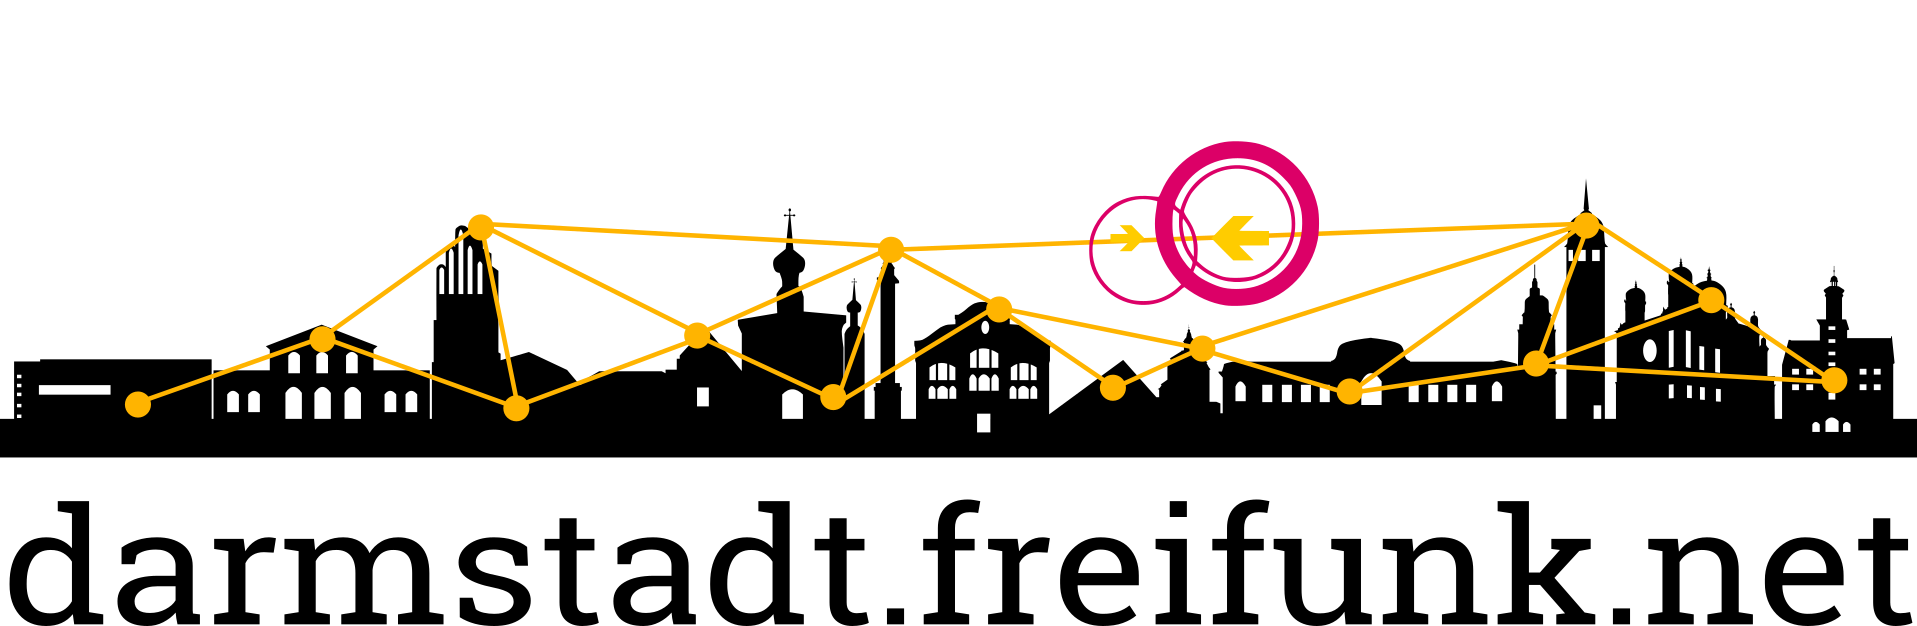
\includegraphics[width=0.6\textwidth]{images/logo-skyline-text-below}
			\vspace{1.4cm}
		\end{center}
			\flushright
			
\includegraphics[width=0.15\textwidth]{images/cda}
	\end{titleframe}
	
	\begin{frame}
		\frametitle{Einleitung}
		\vfill
		\textbf{Was ist Freifunk?}
		\vfill
		\begin{itemize}
			\item nichtkommerzielle Initiative
			\item Ziel: Aufbau und Betrieb eines freien WLAN-Meshnetzes
			\item dezentrales Netz besteht aus den Routern vieler einzelner Betreiber
			\item über 30.000 Freifunk-Router in Deutschland, davon rund 400 in Darmstadt
			\item auf OpenWrt basierte Firmware
		\end{itemize}
		\vfill
		\pause
		Um unkompliziert eigene Services im Freifunk-Netz anbieten zu können, soll im Rahmen dieses Projekts ein Dienst erstellt werden, der das einfache Publizieren und Entdecken verfügbarer Services für den Benutzer übernimmt.
	\end{frame}

	\begin{frame}
		\frametitle{Die Idee (1/7)}
		\begin{center}
			\vspace{0cm}
			\includegraphics[width=0.8\textwidth]{images/service-discovery1}
			\vspace{0.4cm}
		\end{center}

	\end{frame}
	\begin{frame}
		\frametitle{Die Idee (2/7)}
		\begin{center}
			\vspace{0cm}
			\includegraphics[width=0.8\textwidth]{images/service-discovery2}
			\vspace{0.4cm}
		\end{center}
		
	\end{frame}

	\begin{frame}
		\frametitle{Die Idee (3/7)}
		\begin{center}
			\vspace{0cm}
			\includegraphics[width=0.8\textwidth]{images/service-discovery3}
			\vspace{0.4cm}
		\end{center}
		
	\end{frame}
	
	\begin{frame}
		\frametitle{Die Idee (4/7)}
		\begin{center}
			\vspace{0cm}
			\includegraphics[width=0.8\textwidth]{images/service-discovery4}
			\vspace{0.4cm}
		\end{center}
		
	\end{frame}
	\begin{frame}
		\frametitle{Die Idee (5/7)}
		\begin{center}
			\vspace{0cm}
			\includegraphics[width=0.8\textwidth]{images/service-discovery5}
			\vspace{0.4cm}
		\end{center}
		
	\end{frame}
	\begin{frame}
		\frametitle{Die Idee (6/7)}
		\begin{center}
			\vspace{0cm}
			
\includegraphics[width=0.8\textwidth]{images/service-discovery6}
			\vspace{0.4cm}
		\end{center}
		
	\end{frame}
	\begin{frame}
		\frametitle{Die Idee (7/7)}
		\begin{center}
			\vspace{0cm}
			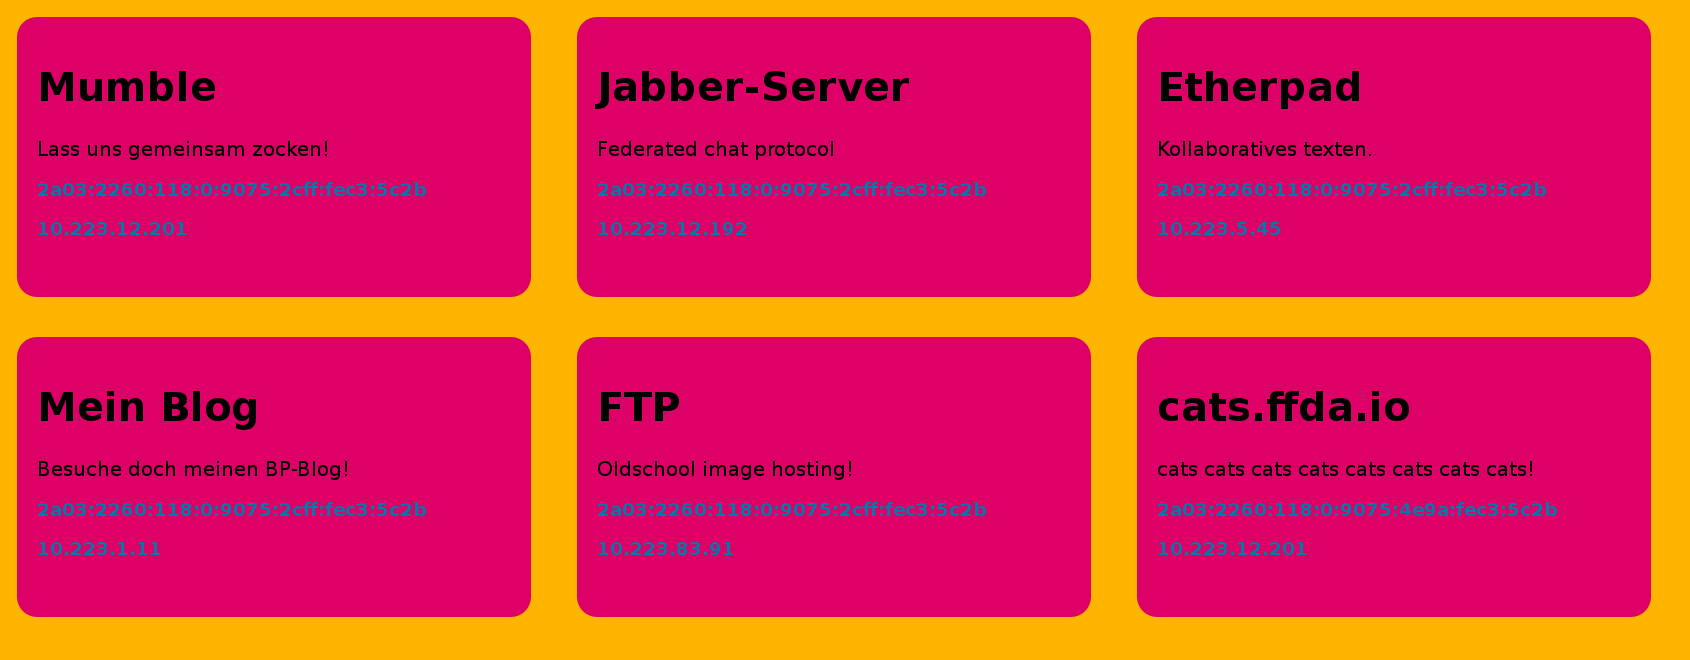
\includegraphics[width=0.8\textwidth]{images/service-discovery7}
			\vspace{0.4cm}
		\end{center}
		
	\end{frame}
	\begin{frame}
		\frametitle{Aufgabenstellung (1/2)}
			Entwicklung eines dezentralen Publish- und Discovery-Dienstes, welcher auf Freifunk-Routern ausgeführt wird.
			\vfill
			\pause
			Dafür werden folgende Komponenten benötigt:
			\begin{itemize}
			\item Endpunkt zum Registrieren von Serviceangeboten
			\item Synchronisation vorhandener Serviceangebote mit Relays im gesamten Netzwerk
			\item zusätzlicher zentraler Verzeichnisdienst
			\end{itemize}
			\vfill
			\pause
			Zur Unterstützung der Entwicklung und für Funktionstests werden zwei WiFi-Router mit der lokalen Freifunk-Firmware bereitgestellt.
	\end{frame}
	
	\begin{frame}
		\frametitle{Aufgabenstellung (2/2)}
		\vfill
		Vorgaben zur Realisierung
		\begin{itemize}
			\item als Programmiersprache C oder C++
			\item Paketierung für OpenWRT-basierte Systeme (opkg)
			\item unter Revisionskontrolle mit Git und sprechenden Commit-Messages\footnote{vgl. \url{http://chris.beams.io/posts/git-commit/}}
			\item lizensiert unter MIT, LGPL oder vergleichbaren Lizenzen
		\end{itemize}
		\vfill
		\pause
		Die Kommunikation zwischen Router und Server, sowie der Router untereinander soll über wohldefinierte, leicht erweiterbare und gut dokumentierte Schnittstellen erfolgen.
		\vfill
	\end{frame}
	
	\begin{frame}
		\frametitle{Fragen?}
			\begin{center}
				\vspace{1cm}
				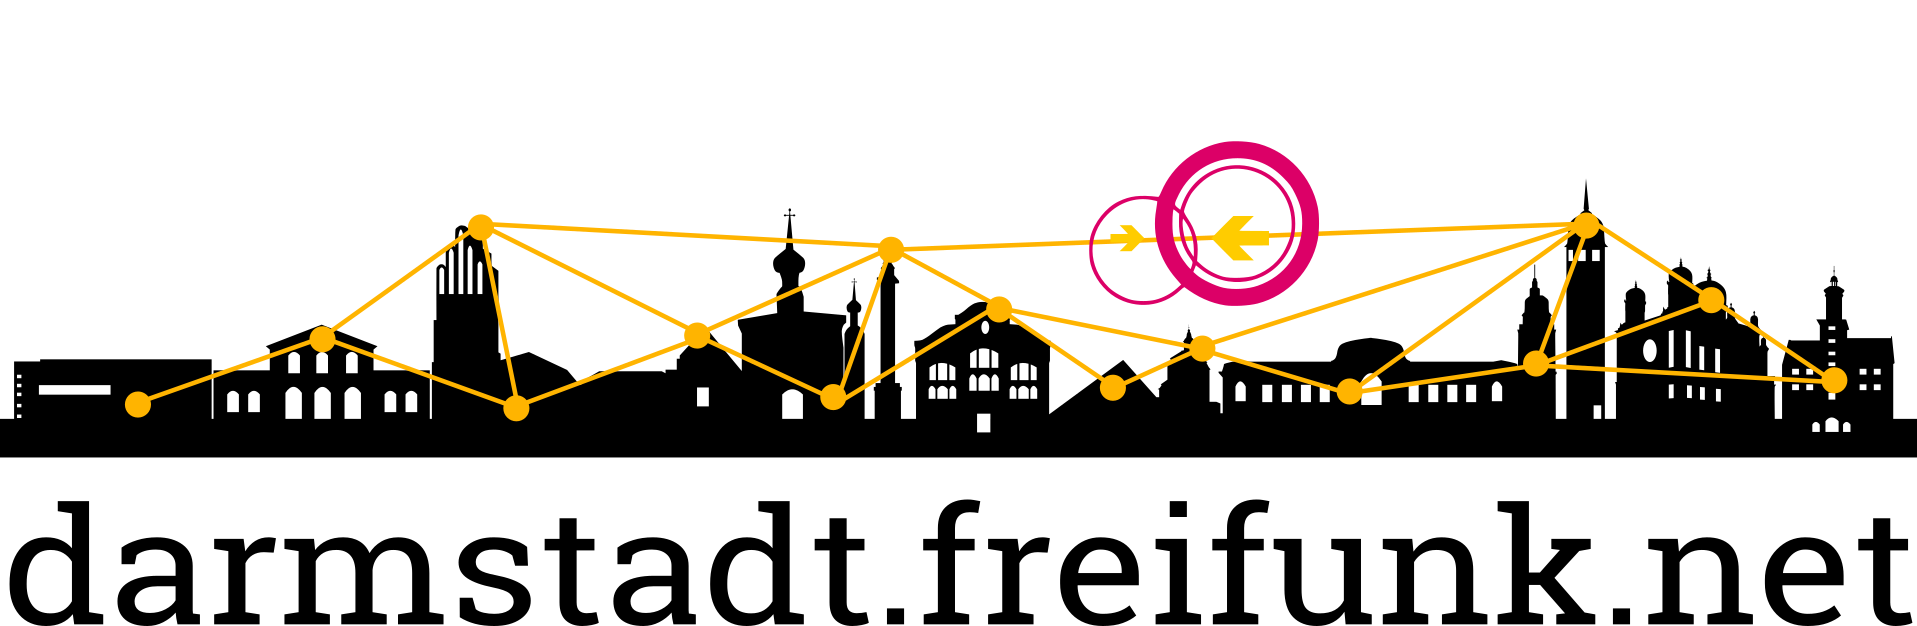
\includegraphics[width=0.6\textwidth]{images/logo-skyline-text-below}
				\vspace{0.6cm}
				bachelorpraktikum@darmstadt.freifunk.net
			\end{center}
		    \vfill
		    
		    
	\end{frame}

\end{document}
